\documentclass[1p]{elsarticle_modified}
%\bibliographystyle{elsarticle-num}

%\usepackage[colorlinks]{hyperref}
%\usepackage{abbrmath_seonhwa} %\Abb, \Ascr, \Acal ,\Abf, \Afrak
\usepackage{amsfonts}
\usepackage{amssymb}
\usepackage{amsmath}
\usepackage{amsthm}
\usepackage{scalefnt}
\usepackage{amsbsy}
\usepackage{kotex}
\usepackage{caption}
\usepackage{subfig}
\usepackage{color}
\usepackage{graphicx}
\usepackage{xcolor} %% white, black, red, green, blue, cyan, magenta, yellow
\usepackage{float}
\usepackage{setspace}
\usepackage{hyperref}

\usepackage{tikz}
\usetikzlibrary{arrows}

\usepackage{multirow}
\usepackage{array} % fixed length table
\usepackage{hhline}

%%%%%%%%%%%%%%%%%%%%%
\makeatletter
\renewcommand*\env@matrix[1][\arraystretch]{%
	\edef\arraystretch{#1}%
	\hskip -\arraycolsep
	\let\@ifnextchar\new@ifnextchar
	\array{*\c@MaxMatrixCols c}}
\makeatother %https://tex.stackexchange.com/questions/14071/how-can-i-increase-the-line-spacing-in-a-matrix
%%%%%%%%%%%%%%%

\usepackage[normalem]{ulem}

\newcommand{\msout}[1]{\ifmmode\text{\sout{\ensuremath{#1}}}\else\sout{#1}\fi}
%SOURCE: \msout is \stkout macro in https://tex.stackexchange.com/questions/20609/strikeout-in-math-mode

\newcommand{\cancel}[1]{
	\ifmmode
	{\color{red}\msout{#1}}
	\else
	{\color{red}\sout{#1}}
	\fi
}

\newcommand{\add}[1]{
	{\color{blue}\uwave{#1}}
}

\newcommand{\replace}[2]{
	\ifmmode
	{\color{red}\msout{#1}}{\color{blue}\uwave{#2}}
	\else
	{\color{red}\sout{#1}}{\color{blue}\uwave{#2}}
	\fi
}

\newcommand{\Sol}{\mathcal{S}} %segment
\newcommand{\D}{D} %diagram
\newcommand{\A}{\mathcal{A}} %arc


%%%%%%%%%%%%%%%%%%%%%%%%%%%%%5 test

\def\sl{\operatorname{\textup{SL}}(2,\Cbb)}
\def\psl{\operatorname{\textup{PSL}}(2,\Cbb)}
\def\quan{\mkern 1mu \triangleright \mkern 1mu}

\theoremstyle{definition}
\newtheorem{thm}{Theorem}[section]
\newtheorem{prop}[thm]{Proposition}
\newtheorem{lem}[thm]{Lemma}
\newtheorem{ques}[thm]{Question}
\newtheorem{cor}[thm]{Corollary}
\newtheorem{defn}[thm]{Definition}
\newtheorem{exam}[thm]{Example}
\newtheorem{rmk}[thm]{Remark}
\newtheorem{alg}[thm]{Algorithm}

\newcommand{\I}{\sqrt{-1}}
\begin{document}

%\begin{frontmatter}
%
%\title{Boundary parabolic representations of knots up to 8 crossings}
%
%%% Group authors per affiliation:
%\author{Yunhi Cho} 
%\address{Department of Mathematics, University of Seoul, Seoul, Korea}
%\ead{yhcho@uos.ac.kr}
%
%
%\author{Seonhwa Kim} %\fnref{s_kim}}
%\address{Center for Geometry and Physics, Institute for Basic Science, Pohang, 37673, Korea}
%\ead{ryeona17@ibs.re.kr}
%
%\author{Hyuk Kim}
%\address{Department of Mathematical Sciences, Seoul National University, Seoul 08826, Korea}
%\ead{hyukkim@snu.ac.kr}
%
%\author{Seokbeom Yoon}
%\address{Department of Mathematical Sciences, Seoul National University, Seoul, 08826,  Korea}
%\ead{sbyoon15@snu.ac.kr}
%
%\begin{abstract}
%We find all boundary parabolic representation of knots up to 8 crossings.
%
%\end{abstract}
%\begin{keyword}
%    \MSC[2010] 57M25 
%\end{keyword}
%
%\end{frontmatter}

%\linenumbers
%\tableofcontents
%
\newcommand\colored[1]{\textcolor{white}{\rule[-0.35ex]{0.8em}{1.4ex}}\kern-0.8em\color{red} #1}%
%\newcommand\colored[1]{\textcolor{white}{ #1}\kern-2.17ex	\textcolor{white}{ #1}\kern-1.81ex	\textcolor{white}{ #1}\kern-2.15ex\color{red}#1	}

{\Large $\underline{11n_{180}~(K11n_{180})}$}

\setlength{\tabcolsep}{10pt}
\renewcommand{\arraystretch}{1.6}
\vspace{1cm}\begin{tabular}{m{100pt}>{\centering\arraybackslash}m{274pt}}
\multirow{5}{120pt}{
	\centering
	\includegraphics[width=112pt]{../../../GIT/diagram.site/Diagrams/png/796_11n_180.png}\\
\ \ \ A knot diagram\footnotemark}&
\allowdisplaybreaks
\textbf{Linearized knot diagam} \\
\cline{2-2}
 &
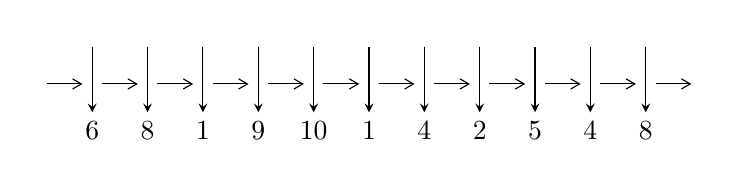
\begin{tikzpicture}[x=20pt, y=17pt]
	% nodes
	\node (C0) at (0, 0) {};
	\node (C1) at (1, 0) {};
	\node (C1U) at (1, +1) {};
	\node (C1D) at (1, -1) {6};

	\node (C2) at (2, 0) {};
	\node (C2U) at (2, +1) {};
	\node (C2D) at (2, -1) {8};

	\node (C3) at (3, 0) {};
	\node (C3U) at (3, +1) {};
	\node (C3D) at (3, -1) {1};

	\node (C4) at (4, 0) {};
	\node (C4U) at (4, +1) {};
	\node (C4D) at (4, -1) {9};

	\node (C5) at (5, 0) {};
	\node (C5U) at (5, +1) {};
	\node (C5D) at (5, -1) {10};

	\node (C6) at (6, 0) {};
	\node (C6U) at (6, +1) {};
	\node (C6D) at (6, -1) {1};

	\node (C7) at (7, 0) {};
	\node (C7U) at (7, +1) {};
	\node (C7D) at (7, -1) {4};

	\node (C8) at (8, 0) {};
	\node (C8U) at (8, +1) {};
	\node (C8D) at (8, -1) {2};

	\node (C9) at (9, 0) {};
	\node (C9U) at (9, +1) {};
	\node (C9D) at (9, -1) {5};

	\node (C10) at (10, 0) {};
	\node (C10U) at (10, +1) {};
	\node (C10D) at (10, -1) {4};

	\node (C11) at (11, 0) {};
	\node (C11U) at (11, +1) {};
	\node (C11D) at (11, -1) {8};
	\node (C12) at (12, 0) {};

	% arrows
	\draw[->,>={angle 60}]
	(C0) edge (C1) (C1) edge (C2) (C2) edge (C3) (C3) edge (C4) (C4) edge (C5) (C5) edge (C6) (C6) edge (C7) (C7) edge (C8) (C8) edge (C9) (C9) edge (C10) (C10) edge (C11) (C11) edge (C12) ;	\draw[->,>=stealth]
	(C1U) edge (C1D) (C2U) edge (C2D) (C3U) edge (C3D) (C4U) edge (C4D) (C5U) edge (C5D) (C6U) edge (C6D) (C7U) edge (C7D) (C8U) edge (C8D) (C9U) edge (C9D) (C10U) edge (C10D) (C11U) edge (C11D) ;
	\end{tikzpicture} \\
\hhline{~~} \\& 
\textbf{Solving Sequence} \\ \cline{2-2} 
 &
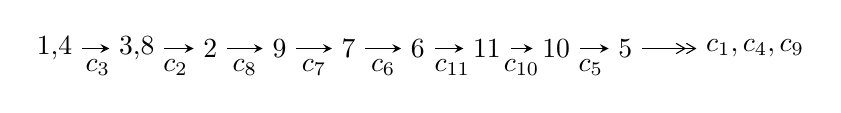
\begin{tikzpicture}[x=25pt, y=7pt]
	% node
	\node (A0) at (-1/8, 0) {1,4};
	\node (A1) at (17/16, 0) {3,8};
	\node (A2) at (17/8, 0) {2};
	\node (A3) at (25/8, 0) {9};
	\node (A4) at (33/8, 0) {7};
	\node (A5) at (41/8, 0) {6};
	\node (A6) at (49/8, 0) {11};
	\node (A7) at (57/8, 0) {10};
	\node (A8) at (65/8, 0) {5};
	\node (C1) at (1/2, -1) {$c_{3}$};
	\node (C2) at (13/8, -1) {$c_{2}$};
	\node (C3) at (21/8, -1) {$c_{8}$};
	\node (C4) at (29/8, -1) {$c_{7}$};
	\node (C5) at (37/8, -1) {$c_{6}$};
	\node (C6) at (45/8, -1) {$c_{11}$};
	\node (C7) at (53/8, -1) {$c_{10}$};
	\node (C8) at (61/8, -1) {$c_{5}$};
	\node (A9) at (10, 0) {$c_{1},c_{4},c_{9}$};

	% edge
	\draw[->,>=stealth]	
	(A0) edge (A1) (A1) edge (A2) (A2) edge (A3) (A3) edge (A4) (A4) edge (A5) (A5) edge (A6) (A6) edge (A7) (A7) edge (A8) ;
	\draw[->>,>={angle 60}]	
	(A8) edge (A9);
\end{tikzpicture} \\ 

\end{tabular} \\

\footnotetext{
The image of knot diagram is generated by the software ``\textbf{Draw programme}" developed by Andrew Bartholomew(\url{http://www.layer8.co.uk/maths/draw/index.htm\#Running-draw}), where we modified some parts for our purpose(\url{https://github.com/CATsTAILs/LinksPainter}).
}\phantom \\ \newline 
\centering \textbf{Ideals for irreducible components\footnotemark of $X_{\text{par}}$} 
 
\begin{align*}
I^u_{1}&=\langle 
4 u^{15}-51 u^{14}+\cdots+4 b-164,\;-41 u^{15}+460 u^{14}+\cdots+32 a+944,\;u^{16}-12 u^{15}+\cdots-360 u^2+32\rangle \\
I^u_{2}&=\langle 
u^8+2 u^7+3 u^2+b+1,\;- u^8-2 u^7+u^6+2 u^5- u^4-2 u^3-2 u^2+a+u,\\
\phantom{I^u_{2}}&\phantom{= \langle  }u^9+3 u^8+u^7-2 u^6+u^5+2 u^4+2 u^3+2 u^2+1\rangle \\
I^u_{3}&=\langle 
39 a^9 u-16 a^8 u+\cdots+108 a+311,\;a^9 u+8 a^8 u+\cdots-58 a+53,\;u^2+u-1\rangle \\
\\
\end{align*}
\raggedright * 3 irreducible components of $\dim_{\mathbb{C}}=0$, with total 45 representations.\\
\footnotetext{All coefficients of polynomials are rational numbers. But the coefficients are sometimes approximated in decimal forms when there is not enough margin.}
\newpage
\renewcommand{\arraystretch}{1}
\centering \section*{I. $I^u_{1}= \langle 4 u^{15}-51 u^{14}+\cdots+4 b-164,\;-41 u^{15}+460 u^{14}+\cdots+32 a+944,\;u^{16}-12 u^{15}+\cdots-360 u^2+32 \rangle$}
\flushleft \textbf{(i) Arc colorings}\\
\begin{tabular}{m{7pt} m{180pt} m{7pt} m{180pt} }
\flushright $a_{1}=$&$\begin{pmatrix}0\\u\end{pmatrix}$ \\
\flushright $a_{4}=$&$\begin{pmatrix}1\\0\end{pmatrix}$ \\
\flushright $a_{3}=$&$\begin{pmatrix}1\\- u^2\end{pmatrix}$ \\
\flushright $a_{8}=$&$\begin{pmatrix}\frac{41}{32} u^{15}-\frac{115}{8} u^{14}+\cdots-17 u-\frac{59}{2}\\- u^{15}+\frac{51}{4} u^{14}+\cdots+\frac{59}{2} u+41\end{pmatrix}$ \\
\flushright $a_{2}=$&$\begin{pmatrix}-\frac{1}{32} u^{15}+\frac{5}{16} u^{14}+\cdots-\frac{45}{8} u^2+1\\\frac{1}{16} u^{15}-\frac{5}{8} u^{14}+\cdots+\frac{41}{4} u^2-1\end{pmatrix}$ \\
\flushright $a_{9}=$&$\begin{pmatrix}\frac{7}{16} u^{15}-\frac{51}{16} u^{14}+\cdots+\frac{47}{4} u+\frac{15}{2}\\-\frac{101}{16} u^{15}+\frac{519}{8} u^{14}+\cdots+\frac{79}{2} u+102\end{pmatrix}$ \\
\flushright $a_{7}=$&$\begin{pmatrix}\frac{9}{32} u^{15}-\frac{13}{8} u^{14}+\cdots+\frac{25}{2} u+\frac{23}{2}\\- u^{15}+\frac{51}{4} u^{14}+\cdots+\frac{59}{2} u+41\end{pmatrix}$ \\
\flushright $a_{6}=$&$\begin{pmatrix}\frac{9}{32} u^{15}-\frac{13}{8} u^{14}+\cdots+\frac{25}{2} u+\frac{23}{2}\\-\frac{11}{2} u^{15}+58 u^{14}+\cdots+\frac{77}{2} u+97\end{pmatrix}$ \\
\flushright $a_{11}=$&$\begin{pmatrix}-\frac{31}{32} u^{15}+\frac{171}{16} u^{14}+\cdots+31 u+31\\\frac{15}{16} u^{15}-\frac{83}{8} u^{14}+\cdots-30 u-31\end{pmatrix}$ \\
\flushright $a_{10}=$&$\begin{pmatrix}-\frac{1}{32} u^{15}+\frac{5}{16} u^{14}+\cdots-\frac{45}{8} u^2+u\\\frac{15}{16} u^{15}-\frac{83}{8} u^{14}+\cdots-30 u-31\end{pmatrix}$ \\
\flushright $a_{5}=$&$\begin{pmatrix}-\frac{33}{16} u^{15}+\frac{41}{2} u^{14}+\cdots+u+26\\\frac{11}{4} u^{15}-\frac{223}{8} u^{14}+\cdots-11 u-40\end{pmatrix}$\\ \flushright $a_{5}=$&$\begin{pmatrix}-\frac{33}{16} u^{15}+\frac{41}{2} u^{14}+\cdots+u+26\\\frac{11}{4} u^{15}-\frac{223}{8} u^{14}+\cdots-11 u-40\end{pmatrix}$\\&\end{tabular}
\flushleft \textbf{(ii) Obstruction class $= -1$}\\~\\
\flushleft \textbf{(iii) Cusp Shapes $= -6 u^{15}+56 u^{14}-242 u^{13}+661 u^{12}-1316 u^{11}+2028 u^{10}-2382 u^9+1918 u^8-581 u^7-1069 u^6+2137 u^5-2069 u^4+1166 u^3-265 u^2-60 u-2$}\\~\\
\newpage\renewcommand{\arraystretch}{1}
\flushleft \textbf{(iv) u-Polynomials at the component}\newline \\
\begin{tabular}{m{50pt}|m{274pt}}
Crossings & \hspace{64pt}u-Polynomials at each crossing \\
\hline $$\begin{aligned}c_{1},c_{2},c_{6}\\c_{8}\end{aligned}$$&$\begin{aligned}
&u^{16}+3 u^{14}+\cdots-3 u-1
\end{aligned}$\\
\hline $$\begin{aligned}c_{3}\end{aligned}$$&$\begin{aligned}
&u^{16}-12 u^{15}+\cdots-360 u^2+32
\end{aligned}$\\
\hline $$\begin{aligned}c_{4},c_{5},c_{9}\end{aligned}$$&$\begin{aligned}
&u^{16}-5 u^{15}+\cdots-10 u-4
\end{aligned}$\\
\hline $$\begin{aligned}c_{7},c_{11}\end{aligned}$$&$\begin{aligned}
&u^{16}+u^{15}+\cdots-4 u-1
\end{aligned}$\\
\hline $$\begin{aligned}c_{10}\end{aligned}$$&$\begin{aligned}
&u^{16}+15 u^{15}+\cdots+1722 u+196
\end{aligned}$\\
\hline
\end{tabular}\\~\\
\newpage\renewcommand{\arraystretch}{1}
\flushleft \textbf{(v) Riley Polynomials at the component}\newline \\
\begin{tabular}{m{50pt}|m{274pt}}
Crossings & \hspace{64pt}Riley Polynomials at each crossing \\
\hline $$\begin{aligned}c_{1},c_{2},c_{6}\\c_{8}\end{aligned}$$&$\begin{aligned}
&y^{16}+6 y^{15}+\cdots-5 y+1
\end{aligned}$\\
\hline $$\begin{aligned}c_{3}\end{aligned}$$&$\begin{aligned}
&y^{16}-10 y^{15}+\cdots-23040 y+1024
\end{aligned}$\\
\hline $$\begin{aligned}c_{4},c_{5},c_{9}\end{aligned}$$&$\begin{aligned}
&y^{16}-15 y^{15}+\cdots-140 y+16
\end{aligned}$\\
\hline $$\begin{aligned}c_{7},c_{11}\end{aligned}$$&$\begin{aligned}
&y^{16}-27 y^{15}+\cdots-36 y+1
\end{aligned}$\\
\hline $$\begin{aligned}c_{10}\end{aligned}$$&$\begin{aligned}
&y^{16}-3 y^{15}+\cdots-394156 y+38416
\end{aligned}$\\
\hline
\end{tabular}\\~\\
\newpage\flushleft \textbf{(vi) Complex Volumes and Cusp Shapes}
$$\begin{array}{c|c|c}  
\text{Solutions to }I^u_{1}& \I (\text{vol} + \sqrt{-1}CS) & \text{Cusp shape}\\
 \hline 
\begin{aligned}
u &= -0.937606\phantom{ +0.000000I} \\
a &= -0.432873\phantom{ +0.000000I} \\
b &= -0.405864\phantom{ +0.000000I}\end{aligned}
 & -5.72940\phantom{ +0.000000I} & -16.4540\phantom{ +0.000000I} \\ \hline\begin{aligned}
u &= \phantom{-}0.646210 + 0.969563 I \\
a &= -0.294430 + 0.642409 I \\
b &= \phantom{-}0.813119 - 0.129662 I\end{aligned}
 & -0.44623 - 2.35749 I & -11.39443 + 1.24540 I \\ \hline\begin{aligned}
u &= \phantom{-}0.646210 - 0.969563 I \\
a &= -0.294430 - 0.642409 I \\
b &= \phantom{-}0.813119 + 0.129662 I\end{aligned}
 & -0.44623 + 2.35749 I & -11.39443 - 1.24540 I \\ \hline\begin{aligned}
u &= \phantom{-}0.132048 + 1.204660 I \\
a &= \phantom{-}0.014404 - 0.499826 I \\
b &= -0.604023 + 0.048649 I\end{aligned}
 & \phantom{-}2.97261 + 1.81783 I & -9.12623 - 4.02809 I \\ \hline\begin{aligned}
u &= \phantom{-}0.132048 - 1.204660 I \\
a &= \phantom{-}0.014404 + 0.499826 I \\
b &= -0.604023 - 0.048649 I\end{aligned}
 & \phantom{-}2.97261 - 1.81783 I & -9.12623 + 4.02809 I \\ \hline\begin{aligned}
u &= \phantom{-}1.312260 + 0.342243 I \\
a &= \phantom{-}1.36980 - 0.44221 I \\
b &= -1.94888 + 0.11150 I\end{aligned}
 & -11.54010 - 0.83768 I & -14.6260 + 5.7551 I \\ \hline\begin{aligned}
u &= \phantom{-}1.312260 - 0.342243 I \\
a &= \phantom{-}1.36980 + 0.44221 I \\
b &= -1.94888 - 0.11150 I\end{aligned}
 & -11.54010 + 0.83768 I & -14.6260 - 5.7551 I \\ \hline\begin{aligned}
u &= -0.27007 + 1.38948 I \\
a &= \phantom{-}0.071515 + 0.368633 I \\
b &= \phantom{-}0.531520 + 0.000186 I\end{aligned}
 & -1.44057 + 5.86096 I & -14.3345 - 7.4758 I \\ \hline\begin{aligned}
u &= -0.27007 - 1.38948 I \\
a &= \phantom{-}0.071515 - 0.368633 I \\
b &= \phantom{-}0.531520 - 0.000186 I\end{aligned}
 & -1.44057 - 5.86096 I & -14.3345 + 7.4758 I \\ \hline\begin{aligned}
u &= \phantom{-}1.45999 + 0.54919 I \\
a &= -1.051980 + 0.234978 I \\
b &= \phantom{-}1.66492 + 0.23467 I\end{aligned}
 & -3.42042 - 3.44951 I & -11.26032 + 2.20716 I\\
 \hline 
 \end{array}$$\newpage$$\begin{array}{c|c|c}  
\text{Solutions to }I^u_{1}& \I (\text{vol} + \sqrt{-1}CS) & \text{Cusp shape}\\
 \hline 
\begin{aligned}
u &= \phantom{-}1.45999 - 0.54919 I \\
a &= -1.051980 - 0.234978 I \\
b &= \phantom{-}1.66492 - 0.23467 I\end{aligned}
 & -3.42042 + 3.44951 I & -11.26032 - 2.20716 I \\ \hline\begin{aligned}
u &= \phantom{-}1.61124 + 0.53845 I \\
a &= \phantom{-}1.041830 - 0.051732 I \\
b &= -1.70649 - 0.47762 I\end{aligned}
 & -2.13858 - 8.47484 I & -10.02725 + 6.22402 I \\ \hline\begin{aligned}
u &= \phantom{-}1.61124 - 0.53845 I \\
a &= \phantom{-}1.041830 + 0.051732 I \\
b &= -1.70649 + 0.47762 I\end{aligned}
 & -2.13858 + 8.47484 I & -10.02725 - 6.22402 I \\ \hline\begin{aligned}
u &= \phantom{-}1.68493 + 0.47840 I \\
a &= -1.090820 - 0.055715 I \\
b &= \phantom{-}1.81129 + 0.61572 I\end{aligned}
 & -7.9978 - 12.6965 I & -13.6924 + 6.6132 I \\ \hline\begin{aligned}
u &= \phantom{-}1.68493 - 0.47840 I \\
a &= -1.090820 + 0.055715 I \\
b &= \phantom{-}1.81129 - 0.61572 I\end{aligned}
 & -7.9978 + 12.6965 I & -13.6924 - 6.6132 I \\ \hline\begin{aligned}
u &= -0.215621\phantom{ +0.000000I} \\
a &= \phantom{-}1.31222\phantom{ +0.000000I} \\
b &= \phantom{-}0.282943\phantom{ +0.000000I}\end{aligned}
 & -0.531160\phantom{ +0.000000I} & -18.6230\phantom{ +0.000000I}\\
 \hline 
 \end{array}$$\newpage\newpage\renewcommand{\arraystretch}{1}
\centering \section*{II. $I^u_{2}= \langle u^8+2 u^7+3 u^2+b+1,\;- u^8-2 u^7+\cdots+a+u,\;u^9+3 u^8+u^7-2 u^6+u^5+2 u^4+2 u^3+2 u^2+1 \rangle$}
\flushleft \textbf{(i) Arc colorings}\\
\begin{tabular}{m{7pt} m{180pt} m{7pt} m{180pt} }
\flushright $a_{1}=$&$\begin{pmatrix}0\\u\end{pmatrix}$ \\
\flushright $a_{4}=$&$\begin{pmatrix}1\\0\end{pmatrix}$ \\
\flushright $a_{3}=$&$\begin{pmatrix}1\\- u^2\end{pmatrix}$ \\
\flushright $a_{8}=$&$\begin{pmatrix}u^8+2 u^7- u^6-2 u^5+u^4+2 u^3+2 u^2- u\\- u^8-2 u^7-3 u^2-1\end{pmatrix}$ \\
\flushright $a_{2}=$&$\begin{pmatrix}- u^8-3 u^7- u^6+2 u^5- u^4-2 u^3-2 u^2-2 u+1\\- u^2+1\end{pmatrix}$ \\
\flushright $a_{9}=$&$\begin{pmatrix}u^8+3 u^7+2 u^6- u^5-2 u^4+u^3+4 u^2+u+1\\u^7+2 u^6- u^5- u^4+2 u^3+u\end{pmatrix}$ \\
\flushright $a_{7}=$&$\begin{pmatrix}- u^6-2 u^5+u^4+2 u^3- u^2- u-1\\- u^8-2 u^7-3 u^2-1\end{pmatrix}$ \\
\flushright $a_{6}=$&$\begin{pmatrix}- u^6-2 u^5+u^4+2 u^3- u^2- u-1\\- u^6-2 u^5+u^4+u^3-2 u^2-1\end{pmatrix}$ \\
\flushright $a_{11}=$&$\begin{pmatrix}u^7+2 u^6- u^5- u^4+2 u^3+2 u\\u^8+2 u^7- u^6- u^5+2 u^4+2 u^2+u\end{pmatrix}$ \\
\flushright $a_{10}=$&$\begin{pmatrix}u^8+3 u^7+u^6-2 u^5+u^4+2 u^3+2 u^2+3 u\\u^8+2 u^7- u^6- u^5+2 u^4+2 u^2+u\end{pmatrix}$ \\
\flushright $a_{5}=$&$\begin{pmatrix}- u^8-2 u^7+u^6+u^5-2 u^4+u^3- u\\u^8+2 u^7- u^6-2 u^5+u^4+2 u^3+2 u^2- u+1\end{pmatrix}$\\ \flushright $a_{5}=$&$\begin{pmatrix}- u^8-2 u^7+u^6+u^5-2 u^4+u^3- u\\u^8+2 u^7- u^6-2 u^5+u^4+2 u^3+2 u^2- u+1\end{pmatrix}$\\&\end{tabular}
\flushleft \textbf{(ii) Obstruction class $= 1$}\\~\\
\flushleft \textbf{(iii) Cusp Shapes $= -4 u^8-9 u^7+3 u^6+10 u^5-5 u^4-5 u^3-4 u^2-2 u-5$}\\~\\
\newpage\renewcommand{\arraystretch}{1}
\flushleft \textbf{(iv) u-Polynomials at the component}\newline \\
\begin{tabular}{m{50pt}|m{274pt}}
Crossings & \hspace{64pt}u-Polynomials at each crossing \\
\hline $$\begin{aligned}c_{1},c_{8}\end{aligned}$$&$\begin{aligned}
&u^9+3 u^7+u^6+2 u^5+2 u^4- u^3+u^2- u-1
\end{aligned}$\\
\hline $$\begin{aligned}c_{2},c_{6}\end{aligned}$$&$\begin{aligned}
&u^9+3 u^7- u^6+2 u^5-2 u^4- u^3- u^2- u+1
\end{aligned}$\\
\hline $$\begin{aligned}c_{3}\end{aligned}$$&$\begin{aligned}
&u^9+3 u^8+u^7-2 u^6+u^5+2 u^4+2 u^3+2 u^2+1
\end{aligned}$\\
\hline $$\begin{aligned}c_{4},c_{5}\end{aligned}$$&$\begin{aligned}
&u^9-5 u^7+8 u^5+u^4-3 u^3-2 u^2-2 u+1
\end{aligned}$\\
\hline $$\begin{aligned}c_{7},c_{11}\end{aligned}$$&$\begin{aligned}
&u^9- u^8- u^7- u^6-2 u^5+2 u^4- u^3+3 u^2+1
\end{aligned}$\\
\hline $$\begin{aligned}c_{9}\end{aligned}$$&$\begin{aligned}
&u^9-5 u^7+8 u^5- u^4-3 u^3+2 u^2-2 u-1
\end{aligned}$\\
\hline $$\begin{aligned}c_{10}\end{aligned}$$&$\begin{aligned}
&u^9- u^7+8 u^6-4 u^5+5 u^4-2 u^3+3 u^2-2 u-1
\end{aligned}$\\
\hline
\end{tabular}\\~\\
\newpage\renewcommand{\arraystretch}{1}
\flushleft \textbf{(v) Riley Polynomials at the component}\newline \\
\begin{tabular}{m{50pt}|m{274pt}}
Crossings & \hspace{64pt}Riley Polynomials at each crossing \\
\hline $$\begin{aligned}c_{1},c_{2},c_{6}\\c_{8}\end{aligned}$$&$\begin{aligned}
&y^9+6 y^8+13 y^7+9 y^6-8 y^5-16 y^4-5 y^3+5 y^2+3 y-1
\end{aligned}$\\
\hline $$\begin{aligned}c_{3}\end{aligned}$$&$\begin{aligned}
&y^9-7 y^8+15 y^7-10 y^6+y^5+2 y^4-8 y^2-4 y-1
\end{aligned}$\\
\hline $$\begin{aligned}c_{4},c_{5},c_{9}\end{aligned}$$&$\begin{aligned}
&y^9-10 y^8+41 y^7-86 y^6+90 y^5-29 y^4-19 y^3+6 y^2+8 y-1
\end{aligned}$\\
\hline $$\begin{aligned}c_{7},c_{11}\end{aligned}$$&$\begin{aligned}
&y^9-3 y^8-5 y^7+5 y^6+16 y^5+8 y^4-9 y^3-13 y^2-6 y-1
\end{aligned}$\\
\hline $$\begin{aligned}c_{10}\end{aligned}$$&$\begin{aligned}
&y^9-2 y^8-7 y^7-60 y^6-64 y^5-53 y^4+6 y^3+9 y^2+10 y-1
\end{aligned}$\\
\hline
\end{tabular}\\~\\
\newpage\flushleft \textbf{(vi) Complex Volumes and Cusp Shapes}
$$\begin{array}{c|c|c}  
\text{Solutions to }I^u_{2}& \I (\text{vol} + \sqrt{-1}CS) & \text{Cusp shape}\\
 \hline 
\begin{aligned}
u &= \phantom{-}0.901563 + 0.564856 I \\
a &= \phantom{-}0.432004 + 0.508675 I \\
b &= \phantom{-}0.102151 + 0.702622 I\end{aligned}
 & \phantom{-}1.79239 - 1.81153 I & -9.80943 + 3.54546 I \\ \hline\begin{aligned}
u &= \phantom{-}0.901563 - 0.564856 I \\
a &= \phantom{-}0.432004 - 0.508675 I \\
b &= \phantom{-}0.102151 - 0.702622 I\end{aligned}
 & \phantom{-}1.79239 + 1.81153 I & -9.80943 - 3.54546 I \\ \hline\begin{aligned}
u &= -0.291663 + 0.753926 I \\
a &= \phantom{-}0.866867 - 0.853127 I \\
b &= \phantom{-}0.390361 + 0.902380 I\end{aligned}
 & -0.28529 + 4.77597 I & -8.22483 - 4.15931 I \\ \hline\begin{aligned}
u &= -0.291663 - 0.753926 I \\
a &= \phantom{-}0.866867 + 0.853127 I \\
b &= \phantom{-}0.390361 - 0.902380 I\end{aligned}
 & -0.28529 - 4.77597 I & -8.22483 + 4.15931 I \\ \hline\begin{aligned}
u &= -1.27478\phantom{ +0.000000I} \\
a &= \phantom{-}1.49648\phantom{ +0.000000I} \\
b &= -1.90768\phantom{ +0.000000I}\end{aligned}
 & -11.1241\phantom{ +0.000000I} & -11.2460\phantom{ +0.000000I} \\ \hline\begin{aligned}
u &= \phantom{-}0.233182 + 0.559961 I \\
a &= -1.39335 - 0.25566 I \\
b &= -0.181746 - 0.839836 I\end{aligned}
 & \phantom{-}4.84522 + 1.19732 I & -2.35469 - 1.53706 I \\ \hline\begin{aligned}
u &= \phantom{-}0.233182 - 0.559961 I \\
a &= -1.39335 + 0.25566 I \\
b &= -0.181746 + 0.839836 I\end{aligned}
 & \phantom{-}4.84522 - 1.19732 I & -2.35469 + 1.53706 I \\ \hline\begin{aligned}
u &= -1.54182\phantom{ +0.000000I} \\
a &= -0.881123\phantom{ +0.000000I} \\
b &= \phantom{-}1.35854\phantom{ +0.000000I}\end{aligned}
 & -4.17989\phantom{ +0.000000I} & -9.50990\phantom{ +0.000000I} \\ \hline\begin{aligned}
u &= -1.86956\phantom{ +0.000000I} \\
a &= \phantom{-}0.573604\phantom{ +0.000000I} \\
b &= -1.07239\phantom{ +0.000000I}\end{aligned}
 & -7.27021\phantom{ +0.000000I} & -22.4660\phantom{ +0.000000I}\\
 \hline 
 \end{array}$$\newpage\newpage\renewcommand{\arraystretch}{1}
\centering \section*{III. $I^u_{3}= \langle 39 a^9 u-16 a^8 u+\cdots+108 a+311,\;a^9 u+8 a^8 u+\cdots-58 a+53,\;u^2+u-1 \rangle$}
\flushleft \textbf{(i) Arc colorings}\\
\begin{tabular}{m{7pt} m{180pt} m{7pt} m{180pt} }
\flushright $a_{1}=$&$\begin{pmatrix}0\\u\end{pmatrix}$ \\
\flushright $a_{4}=$&$\begin{pmatrix}1\\0\end{pmatrix}$ \\
\flushright $a_{3}=$&$\begin{pmatrix}1\\u-1\end{pmatrix}$ \\
\flushright $a_{8}=$&$\begin{pmatrix}a\\-7.80000 a^{9} u+3.20000 a^{8} u+\cdots-21.6000 a-62.2000\end{pmatrix}$ \\
\flushright $a_{2}=$&$\begin{pmatrix}-5.40000 a^{9} u+5.60000 a^{8} u+\cdots+18.2000 a+40.4000\\- a^2 u+a^2+2 u\end{pmatrix}$ \\
\flushright $a_{9}=$&$\begin{pmatrix}-14 a^9 u+3 a^8 u+\cdots+24 a+48\\-12.8000 a^{9} u+2.20000 a^{8} u+\cdots+13.4000 a+22.8000\end{pmatrix}$ \\
\flushright $a_{7}=$&$\begin{pmatrix}-7.80000 a^{9} u+3.20000 a^{8} u+\cdots-20.6000 a-62.2000\\-7.80000 a^{9} u+3.20000 a^{8} u+\cdots-21.6000 a-62.2000\end{pmatrix}$ \\
\flushright $a_{6}=$&$\begin{pmatrix}-7.80000 a^{9} u+3.20000 a^{8} u+\cdots-20.6000 a-62.2000\\13.4000 a^{9} u-2.60000 a^{8} u+\cdots-19.2000 a-35.4000\end{pmatrix}$ \\
\flushright $a_{11}=$&$\begin{pmatrix}a^2 u\\-8.20000 a^{9} u+10.8000 a^{8} u+\cdots-5.40000 a-28.8000\end{pmatrix}$ \\
\flushright $a_{10}=$&$\begin{pmatrix}-8.20000 a^{9} u+10.8000 a^{8} u+\cdots-5.40000 a-28.8000\\-8.20000 a^{9} u+10.8000 a^{8} u+\cdots-5.40000 a-28.8000\end{pmatrix}$ \\
\flushright $a_{5}=$&$\begin{pmatrix}-3.20000 a^{9} u+4.80000 a^{8} u+\cdots-13.4000 a-30.8000\\-1.60000 a^{9} u+2.40000 a^{8} u+\cdots-7.20000 a-14.4000\end{pmatrix}$\\ \flushright $a_{5}=$&$\begin{pmatrix}-3.20000 a^{9} u+4.80000 a^{8} u+\cdots-13.4000 a-30.8000\\-1.60000 a^{9} u+2.40000 a^{8} u+\cdots-7.20000 a-14.4000\end{pmatrix}$\\&\end{tabular}
\flushleft \textbf{(ii) Obstruction class $= -1$}\\~\\
\flushleft \textbf{(iii) Cusp Shapes $= \frac{92}{5} a^9 u+\frac{172}{5} a^8 u+\cdots-\frac{376}{5} a-\frac{1102}{5}$}\\~\\
\newpage\renewcommand{\arraystretch}{1}
\flushleft \textbf{(iv) u-Polynomials at the component}\newline \\
\begin{tabular}{m{50pt}|m{274pt}}
Crossings & \hspace{64pt}u-Polynomials at each crossing \\
\hline $$\begin{aligned}c_{1},c_{2},c_{6}\\c_{8}\end{aligned}$$&$\begin{aligned}
&u^{20}- u^{19}+\cdots-42 u-1
\end{aligned}$\\
\hline $$\begin{aligned}c_{3}\end{aligned}$$&$\begin{aligned}
&(u^2+u-1)^{10}
\end{aligned}$\\
\hline $$\begin{aligned}c_{4},c_{5},c_{9}\end{aligned}$$&$\begin{aligned}
&(u^5+u^4-2 u^3- u^2+u-1)^4
\end{aligned}$\\
\hline $$\begin{aligned}c_{7},c_{11}\end{aligned}$$&$\begin{aligned}
&u^{20}+u^{19}+\cdots+40 u-29
\end{aligned}$\\
\hline $$\begin{aligned}c_{10}\end{aligned}$$&$\begin{aligned}
&(u^5-3 u^4+4 u^3- u^2- u+1)^4
\end{aligned}$\\
\hline
\end{tabular}\\~\\
\newpage\renewcommand{\arraystretch}{1}
\flushleft \textbf{(v) Riley Polynomials at the component}\newline \\
\begin{tabular}{m{50pt}|m{274pt}}
Crossings & \hspace{64pt}Riley Polynomials at each crossing \\
\hline $$\begin{aligned}c_{1},c_{2},c_{6}\\c_{8}\end{aligned}$$&$\begin{aligned}
&y^{20}+7 y^{19}+\cdots-1772 y+1
\end{aligned}$\\
\hline $$\begin{aligned}c_{3}\end{aligned}$$&$\begin{aligned}
&(y^2-3 y+1)^{10}
\end{aligned}$\\
\hline $$\begin{aligned}c_{4},c_{5},c_{9}\end{aligned}$$&$\begin{aligned}
&(y^5-5 y^4+8 y^3-3 y^2- y-1)^4
\end{aligned}$\\
\hline $$\begin{aligned}c_{7},c_{11}\end{aligned}$$&$\begin{aligned}
&y^{20}-13 y^{19}+\cdots-12736 y+841
\end{aligned}$\\
\hline $$\begin{aligned}c_{10}\end{aligned}$$&$\begin{aligned}
&(y^5- y^4+8 y^3-3 y^2+3 y-1)^4
\end{aligned}$\\
\hline
\end{tabular}\\~\\
\newpage\flushleft \textbf{(vi) Complex Volumes and Cusp Shapes}
$$\begin{array}{c|c|c}  
\text{Solutions to }I^u_{3}& \I (\text{vol} + \sqrt{-1}CS) & \text{Cusp shape}\\
 \hline 
\begin{aligned}
u &= \phantom{-}0.618034\phantom{ +0.000000I} \\
a &= \phantom{-}0.677607 + 0.002824 I \\
b &= -0.129907 + 1.332380 I\end{aligned}
 & \phantom{-}3.61874 - 1.53058 I & -10.51511 + 4.43065 I \\ \hline\begin{aligned}
u &= \phantom{-}0.618034\phantom{ +0.000000I} \\
a &= \phantom{-}0.677607 - 0.002824 I \\
b &= -0.129907 - 1.332380 I\end{aligned}
 & \phantom{-}3.61874 + 1.53058 I & -10.51511 - 4.43065 I \\ \hline\begin{aligned}
u &= \phantom{-}0.618034\phantom{ +0.000000I} \\
a &= -1.147360 + 0.672981 I \\
b &= \phantom{-}0.02823 - 1.52596 I\end{aligned}
 & -1.92472 - 4.40083 I & -14.7443 + 3.4986 I \\ \hline\begin{aligned}
u &= \phantom{-}0.618034\phantom{ +0.000000I} \\
a &= -1.147360 - 0.672981 I \\
b &= \phantom{-}0.02823 + 1.52596 I\end{aligned}
 & -1.92472 + 4.40083 I & -14.7443 - 3.4986 I \\ \hline\begin{aligned}
u &= \phantom{-}0.618034\phantom{ +0.000000I} \\
a &= -1.00379 + 1.46626 I \\
b &= \phantom{-}0.620375 + 0.906196 I\end{aligned}
 & \phantom{-}1.54676\phantom{ +0.000000I} & -11.48114 + 0. I\phantom{ +0.000000I} \\ \hline\begin{aligned}
u &= \phantom{-}0.618034\phantom{ +0.000000I} \\
a &= -1.00379 - 1.46626 I \\
b &= \phantom{-}0.620375 - 0.906196 I\end{aligned}
 & \phantom{-}1.54676\phantom{ +0.000000I} & -11.48114 + 0. I\phantom{ +0.000000I} \\ \hline\begin{aligned}
u &= \phantom{-}0.618034\phantom{ +0.000000I} \\
a &= \phantom{-}0.21019 + 2.15583 I \\
b &= -0.418784 + 0.001745 I\end{aligned}
 & \phantom{-}3.61874 + 1.53058 I & -10.51511 - 4.43065 I \\ \hline\begin{aligned}
u &= \phantom{-}0.618034\phantom{ +0.000000I} \\
a &= \phantom{-}0.21019 - 2.15583 I \\
b &= -0.418784 - 0.001745 I\end{aligned}
 & \phantom{-}3.61874 - 1.53058 I & -10.51511 + 4.43065 I \\ \hline\begin{aligned}
u &= \phantom{-}0.618034\phantom{ +0.000000I} \\
a &= -0.04567 + 2.46906 I \\
b &= \phantom{-}0.709108 - 0.415925 I\end{aligned}
 & -1.92472 - 4.40083 I & -14.7443 + 3.4986 I \\ \hline\begin{aligned}
u &= \phantom{-}0.618034\phantom{ +0.000000I} \\
a &= -0.04567 - 2.46906 I \\
b &= \phantom{-}0.709108 + 0.415925 I\end{aligned}
 & -1.92472 + 4.40083 I & -14.7443 - 3.4986 I\\
 \hline 
 \end{array}$$\newpage$$\begin{array}{c|c|c}  
\text{Solutions to }I^u_{3}& \I (\text{vol} + \sqrt{-1}CS) & \text{Cusp shape}\\
 \hline 
\begin{aligned}
u &= -1.61803\phantom{ +0.000000I} \\
a &= \phantom{-}0.972088 + 0.050869 I \\
b &= -1.36329 + 0.42595 I\end{aligned}
 & -4.27694 + 1.53058 I & -10.51511 - 4.43065 I \\ \hline\begin{aligned}
u &= -1.61803\phantom{ +0.000000I} \\
a &= \phantom{-}0.972088 - 0.050869 I \\
b &= -1.36329 - 0.42595 I\end{aligned}
 & -4.27694 - 1.53058 I & -10.51511 + 4.43065 I \\ \hline\begin{aligned}
u &= -1.61803\phantom{ +0.000000I} \\
a &= \phantom{-}0.950790 + 0.411274 I \\
b &= -1.82005 + 0.07628 I\end{aligned}
 & -9.82040 - 4.40083 I & -14.7443 + 3.4986 I \\ \hline\begin{aligned}
u &= -1.61803\phantom{ +0.000000I} \\
a &= \phantom{-}0.950790 - 0.411274 I \\
b &= -1.82005 - 0.07628 I\end{aligned}
 & -9.82040 + 4.40083 I & -14.7443 - 3.4986 I \\ \hline\begin{aligned}
u &= -1.61803\phantom{ +0.000000I} \\
a &= -0.842560 + 0.263250 I \\
b &= \phantom{-}1.57287 + 0.08231 I\end{aligned}
 & -4.27694 + 1.53058 I & -10.51511 - 4.43065 I \\ \hline\begin{aligned}
u &= -1.61803\phantom{ +0.000000I} \\
a &= -0.842560 - 0.263250 I \\
b &= \phantom{-}1.57287 - 0.08231 I\end{aligned}
 & -4.27694 - 1.53058 I & -10.51511 + 4.43065 I \\ \hline\begin{aligned}
u &= -1.61803\phantom{ +0.000000I} \\
a &= -1.124850 + 0.047143 I \\
b &= \phantom{-}1.53841 + 0.66546 I\end{aligned}
 & -9.82040 - 4.40083 I & -14.7443 + 3.4986 I \\ \hline\begin{aligned}
u &= -1.61803\phantom{ +0.000000I} \\
a &= -1.124850 - 0.047143 I \\
b &= \phantom{-}1.53841 - 0.66546 I\end{aligned}
 & -9.82040 + 4.40083 I & -14.7443 - 3.4986 I \\ \hline\begin{aligned}
u &= -1.61803\phantom{ +0.000000I} \\
a &= -0.790561\phantom{ +0.000000I} \\
b &= \phantom{-}0.805229\phantom{ +0.000000I}\end{aligned}
 & -6.34892\phantom{ +0.000000I} & -11.4810\phantom{ +0.000000I} \\ \hline\begin{aligned}
u &= -1.61803\phantom{ +0.000000I} \\
a &= \phantom{-}0.497659\phantom{ +0.000000I} \\
b &= -1.27915\phantom{ +0.000000I}\end{aligned}
 & -6.34892\phantom{ +0.000000I} & -11.4810\phantom{ +0.000000I}\\
 \hline 
 \end{array}$$\newpage
\newpage\renewcommand{\arraystretch}{1}
\centering \section*{ IV. u-Polynomials}
\begin{tabular}{m{50pt}|m{274pt}}
Crossings & \hspace{64pt}u-Polynomials at each crossing \\
\hline $$\begin{aligned}c_{1},c_{8}\end{aligned}$$&$\begin{aligned}
&(u^9+3 u^7+\cdots- u-1)(u^{16}+3 u^{14}+\cdots-3 u-1)\\
&\cdot(u^{20}- u^{19}+\cdots-42 u-1)
\end{aligned}$\\
\hline $$\begin{aligned}c_{2},c_{6}\end{aligned}$$&$\begin{aligned}
&(u^9+3 u^7+\cdots- u+1)(u^{16}+3 u^{14}+\cdots-3 u-1)\\
&\cdot(u^{20}- u^{19}+\cdots-42 u-1)
\end{aligned}$\\
\hline $$\begin{aligned}c_{3}\end{aligned}$$&$\begin{aligned}
&(u^2+u-1)^{10}(u^9+3 u^8+u^7-2 u^6+u^5+2 u^4+2 u^3+2 u^2+1)\\
&\cdot(u^{16}-12 u^{15}+\cdots-360 u^2+32)
\end{aligned}$\\
\hline $$\begin{aligned}c_{4},c_{5}\end{aligned}$$&$\begin{aligned}
&((u^5+u^4-2 u^3- u^2+u-1)^4)(u^9-5 u^7+\cdots-2 u+1)\\
&\cdot(u^{16}-5 u^{15}+\cdots-10 u-4)
\end{aligned}$\\
\hline $$\begin{aligned}c_{7},c_{11}\end{aligned}$$&$\begin{aligned}
&(u^9- u^8+\cdots+3 u^2+1)(u^{16}+u^{15}+\cdots-4 u-1)\\
&\cdot(u^{20}+u^{19}+\cdots+40 u-29)
\end{aligned}$\\
\hline $$\begin{aligned}c_{9}\end{aligned}$$&$\begin{aligned}
&((u^5+u^4-2 u^3- u^2+u-1)^4)(u^9-5 u^7+\cdots-2 u-1)\\
&\cdot(u^{16}-5 u^{15}+\cdots-10 u-4)
\end{aligned}$\\
\hline $$\begin{aligned}c_{10}\end{aligned}$$&$\begin{aligned}
&(u^5-3 u^4+4 u^3- u^2- u+1)^4\\
&\cdot(u^9- u^7+8 u^6-4 u^5+5 u^4-2 u^3+3 u^2-2 u-1)\\
&\cdot(u^{16}+15 u^{15}+\cdots+1722 u+196)
\end{aligned}$\\
\hline
\end{tabular}\newpage\renewcommand{\arraystretch}{1}
\centering \section*{ V. Riley Polynomials}
\begin{tabular}{m{50pt}|m{274pt}}
Crossings & \hspace{64pt}Riley Polynomials at each crossing \\
\hline $$\begin{aligned}c_{1},c_{2},c_{6}\\c_{8}\end{aligned}$$&$\begin{aligned}
&(y^9+6 y^8+13 y^7+9 y^6-8 y^5-16 y^4-5 y^3+5 y^2+3 y-1)\\
&\cdot(y^{16}+6 y^{15}+\cdots-5 y+1)(y^{20}+7 y^{19}+\cdots-1772 y+1)
\end{aligned}$\\
\hline $$\begin{aligned}c_{3}\end{aligned}$$&$\begin{aligned}
&(y^2-3 y+1)^{10}(y^9-7 y^8+15 y^7-10 y^6+y^5+2 y^4-8 y^2-4 y-1)\\
&\cdot(y^{16}-10 y^{15}+\cdots-23040 y+1024)
\end{aligned}$\\
\hline $$\begin{aligned}c_{4},c_{5},c_{9}\end{aligned}$$&$\begin{aligned}
&(y^5-5 y^4+8 y^3-3 y^2- y-1)^4\\
&\cdot(y^9-10 y^8+41 y^7-86 y^6+90 y^5-29 y^4-19 y^3+6 y^2+8 y-1)\\
&\cdot(y^{16}-15 y^{15}+\cdots-140 y+16)
\end{aligned}$\\
\hline $$\begin{aligned}c_{7},c_{11}\end{aligned}$$&$\begin{aligned}
&(y^9-3 y^8-5 y^7+5 y^6+16 y^5+8 y^4-9 y^3-13 y^2-6 y-1)\\
&\cdot(y^{16}-27 y^{15}+\cdots-36 y+1)(y^{20}-13 y^{19}+\cdots-12736 y+841)
\end{aligned}$\\
\hline $$\begin{aligned}c_{10}\end{aligned}$$&$\begin{aligned}
&(y^5- y^4+8 y^3-3 y^2+3 y-1)^4\\
&\cdot(y^9-2 y^8-7 y^7-60 y^6-64 y^5-53 y^4+6 y^3+9 y^2+10 y-1)\\
&\cdot(y^{16}-3 y^{15}+\cdots-394156 y+38416)
\end{aligned}$\\
\hline
\end{tabular}
\vskip 2pc
\end{document}